\section{在线抱怨问题识别}\label{sec:1.3}
\subsection{在线抱怨问题表示结构}\label{subsection:1.3.1}

抱怨问题是抱怨内容反映的产品或服务存在问题的抽象表示,
它主要由抱怨目标、触发短语(触发核心词与相应修饰词)及抱怨问题路径组成:

(1)抱怨目标短语{\itshape Target\/}({\itshape Tar\/})。
作为抱怨目标,抱怨产品或服务及其特征是抱怨问题中抱怨情绪指向的对象,它是抱怨问题不可或缺的部分。
本文将抱怨产品或服务及其特征定义为抱怨目标短语。
如“根本就无法接受短信”中“短信”就是抱怨目标短语。

(2)触发短语{\itshape Problem-Word\/}({\itshape PW\/})。
考虑到描述抱怨产品及其特征的问题状态的触发短语缺乏固定模式,
触发短语的核心词(即描述目标短语问题状态的触发短语的核心词)被定义为触发核心词\textit{Trigger}(\textit{Tri}),
触发核心词及其词修饰该核心词的组合被定义为触发短语。
如“无法接受”是触发短语,“接受”是触发核心词,“无法”是触发核心词的相应修饰词。

(3)抱怨问题路径{\itshape Path\/}。
抱怨目标短语和不考虑修饰词的抱怨核心词的简单组合可形成抱怨问题,
但这样的简单组合忽略了两者间的句法关系(即De Saeger、Tutubalina等人的做法)。
本文将{(触发核心词,相应修饰词),抱怨目标短语}这样的句法关系定义并表示为抱怨问题路径。

根据如上描述,抱怨问题的识别可分解为抱怨目标短语的识别、触发核心词的识别及抱怨问题路径的抽取。
基于此,本文通过引入组成结构分析、依存结构分析和统计学习技术,设计出如\autoref{fig:1.1}所示的识别方法框架。

\begin{figure}[th]

\centering
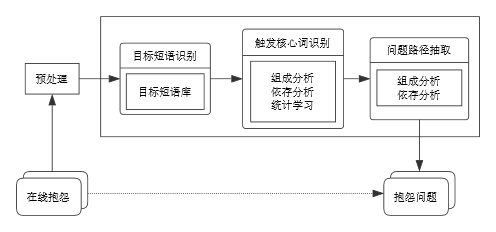
\includegraphics[width=0.9\textwidth]{figure1-1.png}
\vskip -20pt
\caption{在线抱怨问题识别框架}\label{fig:1.1}

\end{figure}

\subsection{抱怨目标短语识别}\label{subsection:1.3.2}

作为抱怨识别的一个重要组成部分,抱怨目标短语识别是后续触发核心词识别和抱怨问题路径抽取的基础。
通常情况下,抱怨目标短语指的是在线抱怨涉及的产品或服务及特征,其中产品特征又分为显性产品特征和隐性产品特征。
显性产品特征即直接出现在产品句子中的产品特征,如“这里信号好差”中的“信号”即为显性产品特征;
隐性产品特征即没有直接出现在句子里、以其他词语描述的间接方式出现的产品特征,
如“啥都没干就用了100M”中的“100M”所描述的手机流量即为隐性产品特征。

在意见挖掘领域,众多学者
(如Kurihara和Shimada\cite{kurihara2015trouble}、Liu等\cite{liu2005opinion}和Lee等\cite{lee2016mining})
为产品特征识别提出了很多不同的方法,
这些方法有效地实现了产品特征的自动抽取,然而它们需要大量难以直接获得的标记数据,且较难直接应用于其他领域。
本文通过搜索领域常用产品及其特征描述的词汇构建抱怨目标短语库,
并根据是否与所建短语库匹配的方式完成抱怨目标短语的识别。

\subsection{触发核心词识别}\label{subsection:1.3.3}
作为抱怨问题识别的关键,触发核心词的识别在抱怨问题识别中具有承上启下的作用,
一则因为触发核心词的存在与抱怨目标相对应,二则触发核心词及相应修饰词是抱怨问题路径抽取的基础。

在触发核心词识别过程中,如何确保抱怨目标短语与所识别的触发核心词相对应是一个不可回避的问题。
为解决这一问题,先将在线抱怨内容分句,进行组成结构分析,以确保抱怨目标短语和触发核心词在同一个句子中;
接着,在进行句法依存分析时,只将句子中与抱怨目标短语存在依存关系的词语作为候选触发核心词,
其他词语不予考虑。在进行这样的预处理后,可作如下假设:

\begin{assumption}\label{assumption:1.1}
    抱怨目标短语和触发核心词在同一个句子中。
\end{assumption}

\begin{assumption}\label{assumption:1.2}
    在句法分析中,触发核心词必须与抱怨目标短语存在依存关系。
\end{assumption}

基于上述假设,可将与抱怨目标短语在同一个句子且存在依存关系的词语确定为候选触发核心词,
再将触发核心词的识别转化为一个二分类问题,并训练一个有监督的高斯核支持向量机(SVM)分类器进行分类。
SVM分类器通过学习触发核心词的特征,
以判定候选触发核心词是否为既定抱怨目标短语对应的触发核心词,从而完成触发核心词的识别。

SVM是Vapnik等\cite{cortes1995support}在统计学习理论基础上提出的有监督的机器学习模型,
它被广泛应用于分类、回归分析及模式识别。
对于二分类,SVM主要通过核函数把原始空间数据向高维特征空间映射,以解决低维空间中线性不可分的问题。
具体地,设$T=\{(x_1,y_1 ),(x_2,y_2 ),\ldots,(x_n,y_n )\}$为训练数据集,
其中$x_i \in X=\mathbb R^N$,\/$y_i \in Y=\{-1,1\}(i=1,2,\ldots,N)$。
若存在向量$\bm w_i$和标量$b$,满足Mercer定理的半正定高斯核函数$K$:
\begin{equation}
    K(x_i,y_i )= \exp(- \frac{\| x_i - y_i \|}{2\delta ^2}) \label{eq:1.1}
\end{equation}

且通过$K$的数据$x_i$从原始输入空间$X$到高维特征空间$F$的映射$\phi(x_i)$满足:
\begin{equation}\label{eq:1.2}
    \begin{cases}
        \boldsymbol{w}^T_i \cdot \phi(x_i) + b \geq 0, & y_i =1 \\
        \boldsymbol{w}^T_i \cdot \phi(x_i) + b < 0, & y_i =-1 
    \end{cases}
\end{equation}

且将分类函数$f(x)$定义为:
\begin{equation}\label{eq:1.3}
    f(x_i) = \boldsymbol{W}^T_i \cdot \phi(x_i) + b
\end{equation}

通过引入松弛变量$\xi_i$和惩罚参数$C$,SVM的最大间隔分类函数可表示为:
\begin{equation}\label{eq:1.4}
    \max \frac{2}{(\| \boldsymbol{w} \| + 2C \sum^N_{i=1} \xi_i)}
\end{equation}

其中$\xi_i \geq 0$且$ y_i (\boldsymbol{w}^T_i \cdot \phi(x_i) + b) \geq 1-\xi_i$。

引入拉格朗日乘子$C \geq \alpha_i \geq 0,i=1,2,3,\ldots,n$,
根据Karush-Kuhn-Tucke条件,将求解\autoref{eq:1.4}最大间隔问题转化为使目标函数$L(\alpha_i)$最大问题:
\begin{equation}\label{eq:1.5}
    \begin{cases}
        \sum^n_{i=1} \alpha_i y_i =0, \alpha_i \geq 0  &\\
        \max\limits_\alpha L(\alpha_i)= \sum^n_{i=1} \alpha_i - \frac 12 \sum^n_{i=1}\sum^n_{j=1} \alpha_i \alpha_j y_i y_j \langle\phi(x_i),\phi(x_j)\rangle & 
    \end{cases}
\end{equation}

最后,通过序列最小最优化SMO算法对拉格朗日乘子$\alpha_i$求解,可解出$\boldsymbol{w}^T_i$和$b$:
\begin{equation}\label{eq:1.6}
    \begin{cases}
        \boldsymbol{w}_i = \sum^n_{i=1} \alpha_i y_i \phi(x_i) & \\
        b=-\frac{\max\limits_{i \colon y_i = -1} (\boldsymbol{w}^T_i \cdot \phi(x_i) ) + \min\limits_{i \colon y_i = 1}(\boldsymbol{w}^T_i \cdot \phi(x_i) )}{2} & 
    \end{cases}
\end{equation}

根据解出的$\boldsymbol{w}_i$和$b$可确定基于训练集$T$的分类函数$f(x)$,并将其用于测试数据的分类。

对于SVM分类特征,可通过包括组成结构分析和依存结构分析在内的句法分析和统计分析获取,
获取后的词语特征如\autoref{tab:1.1}所示。
\begin{table}[ht]
\centering
\caption{词语特征}\label{tab:1.1}
\vskip -10pt
\begin{tabularx}{\textwidth}{cX}
\toprule
特征类型 & 特征描述 \\
\midrule
位置特征$L$ & 是否是第一个词;是否是最后一个词;在句子中的现有位置;与抱怨目标的位置距离 \\
语法特征$Syn$ & 词性;是否是定词;是否是负面词;是否与否定词存在依存关系;是否与负面词存在依存关系;是否与把被让存在依存关系;与抱怨目标依存关系 \\
位置特征$Sta$ & 与抱怨目标的共现次数;在候选触发核心词库中出现的次数 \\
\bottomrule
\end{tabularx}
\end{table}

基于如上叙述,可设计如\autoref{alg:1.1}的触发核心词识别算法:

\begin{algorithm}[htb]
    \SetKwData{Left}{left}\SetKwData{This}{this}\SetKwData{Up}{up}
    \SetKwFunction{Union}{Union}\SetKwFunction{FindCompress}{FindCompress}
\caption{触发核心词识别算法}\label{alg:1.1}

\SetAlgoLined
\KwData{
    抱怨目标短语$Tar$:

    句子的依存结构树$DT=\{ DP,DR \}$;句子的组成结构树$CT=\{CP,CR\}$;

    触发核心词训练集
    $TrainS=\{trains_{L_p};trains_{Syn_p};trains_{Sta_p};R_{(Tar,dp_p )}\}(p=1,2,\ldots,P;R_{(Tar,dp_p )}=-1,1;)$;
    触发核心词测试集$TestS=\{tests_{L_q};tests_{Syn_q};tests_{Sta_q} \} (q=1,2,\ldots,Q; $
    $R_{(Tar,dp_p )}=-1,1)$
}
\KwResult{与抱怨目标Tar对应的触发核心词$Tri$}
\Begin{
    \For{$dp_i$ \textbu{in} $DP$}{
        \If{ $((dr(dp_i,Tar) \in DR) \parallel (dr(Tar,d_i ) \in DR))$ }{
        \textbu{append} $dp_i$ \KwTo $CW$ \;
        }
    }
    \For{$dp_p$ \textbu{in} $CW$}{
        \textbu{append} $\{trains_{L_p};trains_{Syn_p};trains_{Sta_p};R_{(Tar,dp_p )}\}$ \KwTo $Trains$ \textbu{from} $dp_p$ \;
    }
    \emph{\textbu{random select} $trains_q$ \textbu{in} $TrainS$}\;
    \emph{\textbu{trains} \textup{SVM} }\;
}

\end{algorithm}

在\autoref{alg:1.1}的句子依存结构树$DT=\{ DP,DR \}$中,
$DP$为$DT$的节点集合$\{ dp_i \}(i=1,2,⋯,M;dp_m \in Tar;dp_n \in Tri;1 \le m,n \le M)$,
$DR$为节点间的依存关系集合$\{ dr (dp_i,dp_k) \}(i,k=1,2,\ldots,N)$;
在组成结构树$CT=\{CP,CR\}$中,$CP$为组成结构树的节点集合$\{cp_j\}(j=1,2,\ldots,A;cp_a \in Tar;dp_b \in Tri;1 \le a,b \le A)$,
$CR$为节点间的依存关系集合$\{cr (cp_j,cp_s)\}(j,s=1,2,\ldots,B)$,
候选触发核心词集$CW=\{dp_p \}(p=1,2,\ldots,P)$;
在触发核心词训练集$TrainS$中,$trains_{L_p}$、$trains_{Syn_p}$、$trains_{Sta_p}$和$R_{(Tar,dp_p )}$
分别为训练集触发核心词$dp_p$的位置特征、语法特征、统计特征及类别标签;
在触发核心词测试集$TestS$中,$tests_{L_q}$、$tests_{Syn_q}$和$tests_{Sta_q}$
分别为测试集触发核心词$dp_q$的位置特征、语法特征、统计特征及类别标签;

\autoref{alg:1.1}的功能为既定抱怨目标短语识别对应的触发核心词,
它以句子的依存结构、组成结构、抱怨目标短语$Tar$、触发核心词训练集和测试集(输入时为空集,在中间过程附加数据)为输入,
以与抱怨目标短语对应的触发核心词为输出。首先,通过判断与给定的抱怨目标短语是否在同一语句且存在依存关系,
为该抱怨目标短语确定候选触发核心词;
其次,通过组成结构分析、依存结构分析和统计分析获取触发核心词的位置特征、语法特征和统计特征;
再次,将候选触发核心词集汇集为训练集和测试集;
最后,使用训练得到的SVM分类器对候选触发核心词进行分类,若$R_{(Tar,dp_q)}=1$,
则确定$dp_q$为与抱怨目标短语对应的触发核心词Tri,
此时抱怨问题被识别为以该触发核心词为核心的抱怨问题路径。

\subsection{抱怨问题路径抽取}\label{subsection:1.3.4}

为抱怨的核心,抱怨问题通常采用否定或负面词汇来描述抱怨目标短语的问题状况。
因此,如果抱怨目标短语存在问题状况,那么触发核心词要么是否定或负面词,
要么存在否定或负面词修饰触发核心词。相应地,如果触发核心词是否定或负面词,
或者存在否定或负面词修饰触发核心词(即存在特定的依存关系),
那么其所对应的抱怨目标短语极有可能存在问题状况。
另外,为了提高抱怨问题抽取的准确性,本文对双重否定的情况进行了过滤,如果触发核心词是否定或负面词,
且存在否定或负面词修饰该触发核心词,那么抱怨目标短语不存在问题状况。
鉴于此,做出如下假设:
\begin{assumption}\label{assumption:1.3}
    若触发核心词是否定或负面词,且不存在否定或负面词修饰该触发核心词,则抱怨目标短语存在问题状况。
\end{assumption}

\begin{assumption}\label{assumption:1.4}
    若触发核心词是非否定或负面词,但与否定词或负面词存在特定的依存关系,则抱怨目标短语存在问题状况。
\end{assumption}

\begin{assumption}\label{assumption:1.5}
    若触发核心词是否定或负面词,且与否定或负面词存在特定的依存关系,则抱怨目标短语不存在问题状况。
\end{assumption}

在确定抱怨目标短语是否存在问题状况后,如何抽取抱怨问题是接下来的工作。
当触发核心词属于否定或负面词,且不存在否定或负面词修饰该核心词时,
此时的触发核心词就是Gupta\cite{gupta2011extracting}定义的触发短语;当触发核心词属于非否定或负面词,
但与否点或负面词存在特定依存关系时,触发核心词和相应否定或负面修饰词的组合就是触发短语。

鉴于此,本节将抱怨问题表示为由抱怨目标短语、
触发核心词或及触发核心词的相应否定或负面修饰词组成的子树Sub-tree,
从而较好地考虑了三者间的句法关系。
通过判定是否存在与触发核心词存在特定依存关系的否定或负面词以及判定触发核心词是否本身是否定或负面词,
可归纳出如\autoref{fig:1.2}所示的抱怨问题路径抽取流程。

\begin{figure}[th]
    
    \centering
    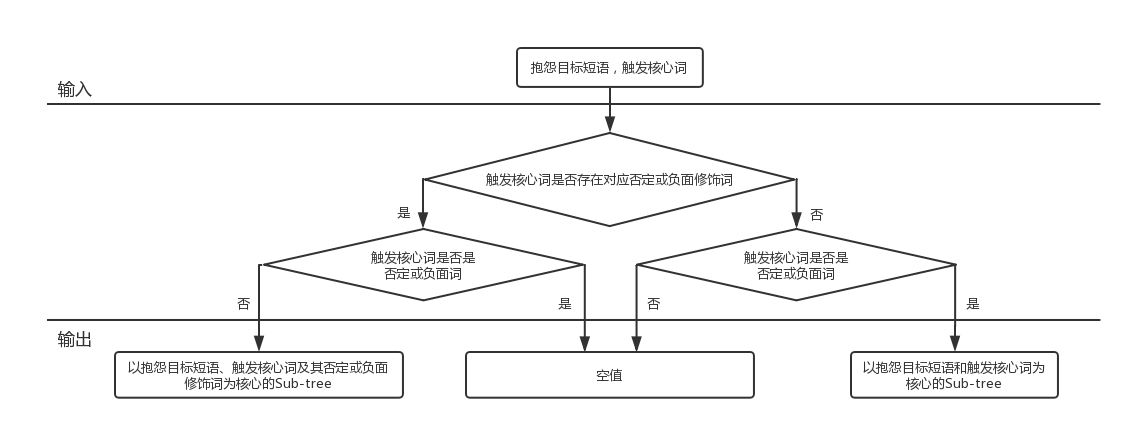
\includegraphics[width=\textwidth]{figure1-2.png}
    \vskip -20pt
    \caption{抱怨问题路径抽取流程}\label{fig:1.2}
\end{figure}

例如,“这里信号好差”中的抱怨目标短语“信号”对应的触发核心词“差”为负面词且无对应否定或负面修饰词,
因此采用由“信号”和“差”组成的Sub-tree来表示抱怨问题;
“根本就无法接受短信”中的抱怨目标短语“短信”对应的触发核心词“接受”为非负面或否定词但存在否定词“无法”对其修饰,
因此采用由“短信”、“接受”和“无法”组成的Sub-tree来表示抱怨问题。

为了更好的表述抱怨问题路径Path的生成过程,这里以在线抱怨“这里根本收不了短信!”为例详细阐述。
应用本章的抱怨目标短语识别方法和触发核心词识别方法,
可识别出本例的抱怨目标短语和触发核心词,分别为“短信”和“收”,该例的抱怨问题路径抽取过程见\autoref{fig:1.3}。

\begin{figure}[th]
    
    \centering
    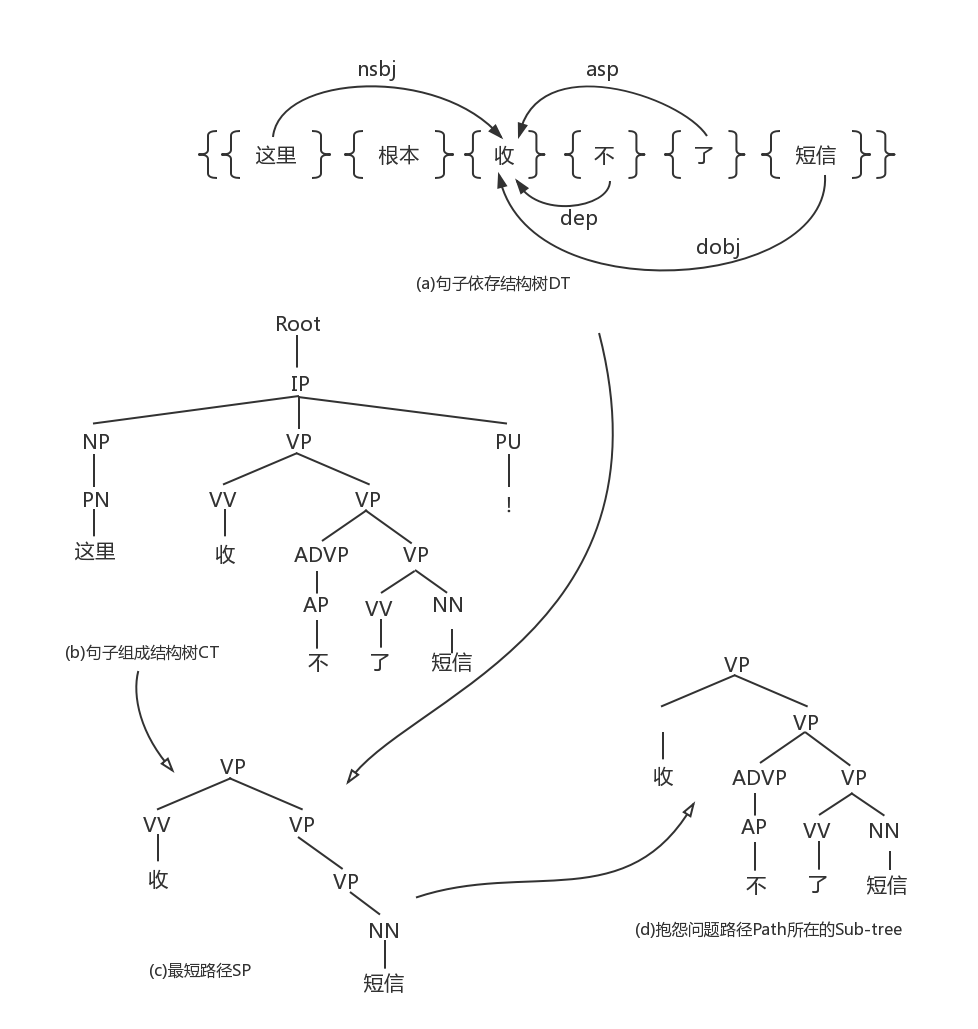
\includegraphics[width=\textwidth]{figure1-3.png}
    \vskip -20pt
    \caption{抱怨问题抽取过程}\label{fig:1.3}
\end{figure}

(1)通过Standford Parser句法分析工具,
获取如\autoref{fig:1.3}(a)和\autoref{fig:1.3}(b)所示的句子依存结构树(CT)和句法组成结构树(DT),
并获取如\autoref{fig:1.3}(c)所示的抱怨目标短语“短信”和触发核心词“收”的最短路径SP;

(2)根据\autoref{fig:1.2}的流程进行判定,可得出抱怨目标短语“短信”和触发核心词“收”外,
DP中与触发核心词“收”存在特定依存关系的有“这里”、“不”、“了”,其中只有“不”属于否定词;

(3)查找负面和否定词词库,得知触发核心词“收”即非负面也非否定词,
故将从“不”到SP根节点“VP”的路径合并到SP中,
再根据组成结构树CT可知抱怨问题路径的结构子树Sub-tree;

(4)返回抱怨问题路径抽取结果“收不了短信”。

